\documentclass[twoside]{book}

% Packages required by doxygen
\usepackage{calc}
\usepackage{doxygen}
\usepackage{graphicx}
\usepackage[utf8]{inputenc}
\usepackage{makeidx}
\usepackage{multicol}
\usepackage{multirow}
\usepackage{textcomp}
\usepackage[table]{xcolor}

% NLS support packages
\usepackage{polski}
\usepackage[T1]{fontenc}

% Font selection
\usepackage[T1]{fontenc}
\usepackage{mathptmx}
\usepackage[scaled=.90]{helvet}
\usepackage{courier}
\usepackage{amssymb}
\usepackage{sectsty}
\renewcommand{\familydefault}{\sfdefault}
\allsectionsfont{%
  \fontseries{bc}\selectfont%
  \color{darkgray}%
}
\renewcommand{\DoxyLabelFont}{%
  \fontseries{bc}\selectfont%
  \color{darkgray}%
}

% Page & text layout
\usepackage{geometry}
\geometry{%
  a4paper,%
  top=2.5cm,%
  bottom=2.5cm,%
  left=2.5cm,%
  right=2.5cm%
}
\tolerance=750
\hfuzz=15pt
\hbadness=750
\setlength{\emergencystretch}{15pt}
\setlength{\parindent}{0cm}
\setlength{\parskip}{0.2cm}
\makeatletter
\renewcommand{\paragraph}{%
  \@startsection{paragraph}{4}{0ex}{-1.0ex}{1.0ex}{%
    \normalfont\normalsize\bfseries\SS@parafont%
  }%
}
\renewcommand{\subparagraph}{%
  \@startsection{subparagraph}{5}{0ex}{-1.0ex}{1.0ex}{%
    \normalfont\normalsize\bfseries\SS@subparafont%
  }%
}
\makeatother

% Headers & footers
\usepackage{fancyhdr}
\pagestyle{fancyplain}
\fancyhead[LE]{\fancyplain{}{\bfseries\thepage}}
\fancyhead[CE]{\fancyplain{}{}}
\fancyhead[RE]{\fancyplain{}{\bfseries\leftmark}}
\fancyhead[LO]{\fancyplain{}{\bfseries\rightmark}}
\fancyhead[CO]{\fancyplain{}{}}
\fancyhead[RO]{\fancyplain{}{\bfseries\thepage}}
\fancyfoot[LE]{\fancyplain{}{}}
\fancyfoot[CE]{\fancyplain{}{}}
\fancyfoot[RE]{\fancyplain{}{\bfseries\scriptsize Wygenerowano Cz, 16 kwi 2015 11\-:26\-:30 dla Optymalizacja działania algorytmów sortowania -\/ Quick Sort programem Doxygen }}
\fancyfoot[LO]{\fancyplain{}{\bfseries\scriptsize Wygenerowano Cz, 16 kwi 2015 11\-:26\-:30 dla Optymalizacja działania algorytmów sortowania -\/ Quick Sort programem Doxygen }}
\fancyfoot[CO]{\fancyplain{}{}}
\fancyfoot[RO]{\fancyplain{}{}}
\renewcommand{\footrulewidth}{0.4pt}
\renewcommand{\chaptermark}[1]{%
  \markboth{#1}{}%
}
\renewcommand{\sectionmark}[1]{%
  \markright{\thesection\ #1}%
}

% Indices & bibliography
\usepackage{natbib}
\usepackage[titles]{tocloft}
\setcounter{tocdepth}{3}
\setcounter{secnumdepth}{5}
\makeindex

% Packages requested by user
\usepackage{graphicx}

% Hyperlinks (required, but should be loaded last)
\usepackage{ifpdf}
\ifpdf
  \usepackage[pdftex,pagebackref=true]{hyperref}
\else
  \usepackage[ps2pdf,pagebackref=true]{hyperref}
\fi
\hypersetup{%
  colorlinks=true,%
  linkcolor=blue,%
  citecolor=blue,%
  unicode%
}

% Custom commands
\newcommand{\clearemptydoublepage}{%
  \newpage{\pagestyle{empty}\cleardoublepage}%
}


%===== C O N T E N T S =====

\begin{document}

% Titlepage & ToC
\hypersetup{pageanchor=false}
\pagenumbering{roman}
\begin{titlepage}
\vspace*{7cm}
\begin{center}%
{\Large Optymalizacja działania algorytmów sortowania -\/ Quick Sort }\\
\vspace*{1cm}
{\large Wygenerowano przez Doxygen 1.8.6}\\
\vspace*{0.5cm}
{\small Cz, 16 kwi 2015 11:26:30}\\
\end{center}
\end{titlepage}
\clearemptydoublepage
\tableofcontents
\clearemptydoublepage
\pagenumbering{arabic}
\hypersetup{pageanchor=true}

%--- Begin generated contents ---
\chapter{Indeks hierarchiczny}
\section{Hierarchia klas}
Ta lista dziedziczenia posortowana jest z grubsza, choć nie całkowicie, alfabetycznie\-:\begin{DoxyCompactList}
\item \contentsline{section}{Benchmark$<$ T $>$}{\pageref{class_benchmark}}{}
\item \contentsline{section}{Lista$<$ T\-Y\-P $>$}{\pageref{class_lista}}{}
\begin{DoxyCompactList}
\item \contentsline{section}{Kolejka$<$ T\-Y\-P $>$}{\pageref{class_kolejka}}{}
\item \contentsline{section}{Stos$<$ T\-Y\-P $>$}{\pageref{class_stos}}{}
\end{DoxyCompactList}
\item \contentsline{section}{Timer}{\pageref{class_timer}}{}
\end{DoxyCompactList}

\chapter{Indeks klas}
\section{Lista klas}
Tutaj znajdują się klasy, struktury, unie i interfejsy wraz z ich krótkimi opisami\-:\begin{DoxyCompactList}
\item\contentsline{section}{\hyperlink{class_benchmark}{Benchmark$<$ T $>$} \\*Klasa do przeprowadzenia testów na kontenerach danych }{\pageref{class_benchmark}}{}
\item\contentsline{section}{\hyperlink{class_kolejka}{Kolejka$<$ T\-Y\-P $>$} \\*Klasa \hyperlink{class_kolejka}{Kolejka} }{\pageref{class_kolejka}}{}
\item\contentsline{section}{\hyperlink{class_lista}{Lista$<$ T\-Y\-P $>$} \\*Klasa \hyperlink{class_lista}{Lista} }{\pageref{class_lista}}{}
\item\contentsline{section}{\hyperlink{class_stos}{Stos$<$ T\-Y\-P $>$} \\*Klasa \hyperlink{class_stos}{Stos} }{\pageref{class_stos}}{}
\item\contentsline{section}{\hyperlink{class_timer}{Timer} \\*Klasa do pomiaru różnicy czasów }{\pageref{class_timer}}{}
\end{DoxyCompactList}

\chapter{Indeks plików}
\section{Lista plików}
Tutaj znajduje się lista wszystkich udokumentowanych plików z ich krótkimi opisami\-:\begin{DoxyCompactList}
\item\contentsline{section}{/home/mateusz/git/209365/\-Lab3/prj/inc/\hyperlink{_benchmark_8hh}{Benchmark.\-hh} \\*Deklaracja i definicja (razem, bo szablon) klasy \hyperlink{class_benchmark}{Benchmark} }{\pageref{_benchmark_8hh}}{}
\item\contentsline{section}{/home/mateusz/git/209365/\-Lab3/prj/inc/\hyperlink{_kolejka_8hh}{Kolejka.\-hh} \\*Definicja klasy \hyperlink{class_kolejka}{Kolejka} }{\pageref{_kolejka_8hh}}{}
\item\contentsline{section}{/home/mateusz/git/209365/\-Lab3/prj/inc/\hyperlink{_lista_8hh}{Lista.\-hh} \\*Definicja klasy \hyperlink{class_lista}{Lista} }{\pageref{_lista_8hh}}{}
\item\contentsline{section}{/home/mateusz/git/209365/\-Lab3/prj/inc/{\bfseries Pivot.\-hh} }{\pageref{_pivot_8hh}}{}
\item\contentsline{section}{/home/mateusz/git/209365/\-Lab3/prj/inc/{\bfseries quick\-\_\-sort.\-hh} }{\pageref{quick__sort_8hh}}{}
\item\contentsline{section}{/home/mateusz/git/209365/\-Lab3/prj/inc/\hyperlink{_stos_8hh}{Stos.\-hh} \\*Definicja klasy \hyperlink{class_stos}{Stos} }{\pageref{_stos_8hh}}{}
\item\contentsline{section}{/home/mateusz/git/209365/\-Lab3/prj/inc/\hyperlink{_timer_8hh}{Timer.\-hh} \\*Plik zawierający deklaracje klasy \hyperlink{class_timer}{Timer} służącej do pomiaru różnicy czasów }{\pageref{_timer_8hh}}{}
\item\contentsline{section}{/home/mateusz/git/209365/\-Lab3/prj/src/\hyperlink{_timer_8cpp}{Timer.\-cpp} \\*Plik zawierający definicje funkcji klasy \hyperlink{class_timer}{Timer} służącej do pomiaru różnicy czasów }{\pageref{_timer_8cpp}}{}
\end{DoxyCompactList}

\chapter{Dokumentacja klas}
\hypertarget{class_benchmark}{\section{Dokumentacja szablonu klasy Benchmark$<$ T $>$}
\label{class_benchmark}\index{Benchmark$<$ T $>$@{Benchmark$<$ T $>$}}
}


Klasa do przeprowadzenia testów na kontenerach danych.  




{\ttfamily \#include $<$Benchmark.\-hh$>$}

\subsection*{Metody publiczne}
\begin{DoxyCompactItemize}
\item 
\hyperlink{class_benchmark_a15ccd21b999908da42c58bd5d127c674}{Benchmark} (unsigned int $\ast$test\-\_\-list\-\_\-sizes, unsigned int size, unsigned int number\-\_\-of\-\_\-memeasurements)
\begin{DoxyCompactList}\small\item\em Konstruktor klasy \hyperlink{class_benchmark}{Benchmark} pomiarający wykładnik liczby określającej dla jakiej liczby elementów testujemy kontener. \end{DoxyCompactList}\item 
\hypertarget{class_benchmark_ac6a294f9ac4fbba06f0a608eb241d3b0}{void {\bfseries test\-Quick\-Sort} (\hyperlink{class_lista}{Lista}$<$ T $>$ $\ast$list, P\-I\-V\-O\-T piv)}\label{class_benchmark_ac6a294f9ac4fbba06f0a608eb241d3b0}

\end{DoxyCompactItemize}


\subsection{Opis szczegółowy}
\subsubsection*{template$<$class T$>$class Benchmark$<$ T $>$}

Klasa do przeprowadzenia testów na kontenerach danych. 

Klasa odpwiada za pomiar czasu koniecznego do umieszczenia określonej liczby danych na stosie, kolejce oraz liście 

\subsection{Dokumentacja konstruktora i destruktora}
\hypertarget{class_benchmark_a15ccd21b999908da42c58bd5d127c674}{\index{Benchmark@{Benchmark}!Benchmark@{Benchmark}}
\index{Benchmark@{Benchmark}!Benchmark@{Benchmark}}
\subsubsection[{Benchmark}]{\setlength{\rightskip}{0pt plus 5cm}template$<$typename T $>$ {\bf Benchmark}$<$ T $>$\-::{\bf Benchmark} (
\begin{DoxyParamCaption}
\item[{unsigned int $\ast$}]{test\-\_\-list\-\_\-sizes, }
\item[{unsigned int}]{size, }
\item[{unsigned int}]{number\-\_\-of\-\_\-memeasurements}
\end{DoxyParamCaption}
)}}\label{class_benchmark_a15ccd21b999908da42c58bd5d127c674}


Konstruktor klasy \hyperlink{class_benchmark}{Benchmark} pomiarający wykładnik liczby określającej dla jakiej liczby elementów testujemy kontener. 


\begin{DoxyParams}{Parametry}
{\em test\-Power} & Liczba określająca wykładnik 10. Cała liczba ( 10$^\wedge$(\-\_\-test\-Power) ) określa liczbe elementów, które będą wkładane do kontenerów.\\
\hline
{\em Liczby} & w tablicy określają jaką ilość danych (jak dużą listę) będziemy kolejno sortować (w celu pomiaru poptrzebnego czasu dla każdej wielkości) \\
\hline
\end{DoxyParams}


Dokumentacja dla tej klasy została wygenerowana z pliku\-:\begin{DoxyCompactItemize}
\item 
/home/mateusz/git/209365/\-Lab3/prj/inc/\hyperlink{_benchmark_8hh}{Benchmark.\-hh}\end{DoxyCompactItemize}

\hypertarget{class_kolejka}{\section{Dokumentacja szablonu klasy Kolejka$<$ T\-Y\-P $>$}
\label{class_kolejka}\index{Kolejka$<$ T\-Y\-P $>$@{Kolejka$<$ T\-Y\-P $>$}}
}


Klasa \hyperlink{class_kolejka}{Kolejka}.  




{\ttfamily \#include $<$Kolejka.\-hh$>$}

Diagram dziedziczenia dla Kolejka$<$ T\-Y\-P $>$\begin{figure}[H]
\begin{center}
\leavevmode
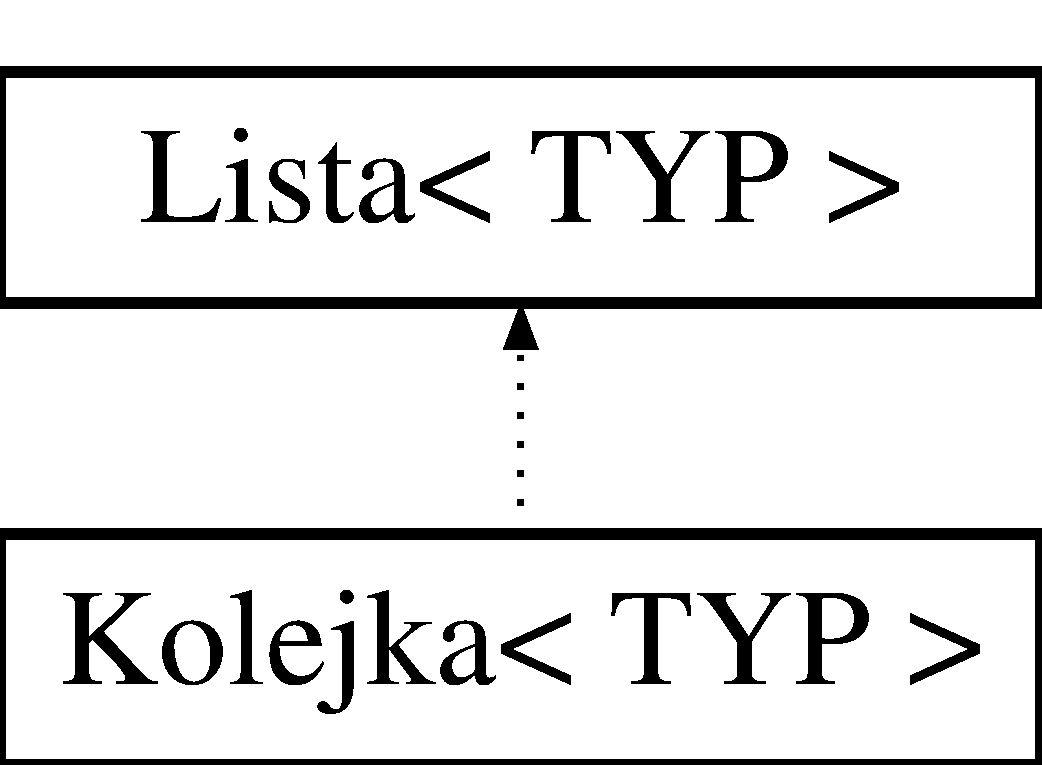
\includegraphics[height=2.000000cm]{class_kolejka}
\end{center}
\end{figure}
\subsection*{Metody publiczne}
\begin{DoxyCompactItemize}
\item 
\hypertarget{class_kolejka_a66056e67a0514466d7771da351e8468b}{void {\bfseries P\-U\-S\-H} (T\-Y\-P liczba)}\label{class_kolejka_a66056e67a0514466d7771da351e8468b}

\item 
\hypertarget{class_kolejka_ab1d8e5d4a855fb2156201a57cc0a9a39}{int {\bfseries P\-O\-P} ()}\label{class_kolejka_ab1d8e5d4a855fb2156201a57cc0a9a39}

\item 
\hypertarget{class_kolejka_a26b5afbcc9f892a41acbd3aed062ee50}{void {\bfseries S\-H\-O\-W} ()}\label{class_kolejka_a26b5afbcc9f892a41acbd3aed062ee50}

\item 
\hypertarget{class_kolejka_a06a7fe157ff434771a700ffd084dc7a2}{unsigned int {\bfseries S\-I\-Z\-E} ()}\label{class_kolejka_a06a7fe157ff434771a700ffd084dc7a2}

\end{DoxyCompactItemize}


\subsection{Opis szczegółowy}
\subsubsection*{template$<$typename T\-Y\-P$>$class Kolejka$<$ T\-Y\-P $>$}

Klasa \hyperlink{class_kolejka}{Kolejka}. 

Klasa ta modeluje nam Kolejke Składa się z pól klasy \hyperlink{class_lista}{Lista} oraz metod P\-U\-S\-H, P\-O\-P, S\-I\-Z\-E, S\-H\-O\-W Klasa w calosci wykorzystuje implementacje listy 

Dokumentacja dla tej klasy została wygenerowana z pliku\-:\begin{DoxyCompactItemize}
\item 
/home/mateusz/git/209365/\-Lab3/prj/inc/\hyperlink{_kolejka_8hh}{Kolejka.\-hh}\end{DoxyCompactItemize}

\hypertarget{class_lista}{\section{Dokumentacja szablonu klasy Lista$<$ T\-Y\-P $>$}
\label{class_lista}\index{Lista$<$ T\-Y\-P $>$@{Lista$<$ T\-Y\-P $>$}}
}


Klasa \hyperlink{class_lista}{Lista}.  




{\ttfamily \#include $<$Lista.\-hh$>$}

Diagram dziedziczenia dla Lista$<$ T\-Y\-P $>$\begin{figure}[H]
\begin{center}
\leavevmode
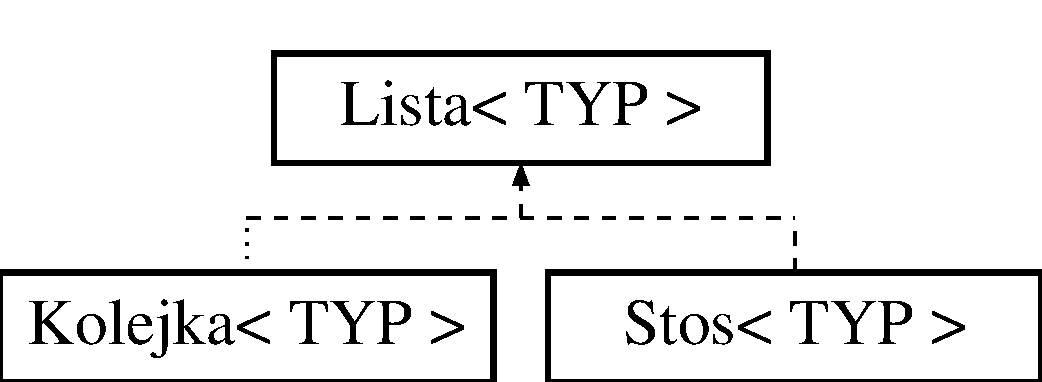
\includegraphics[height=2.000000cm]{class_lista}
\end{center}
\end{figure}
\subsection*{Metody publiczne}
\begin{DoxyCompactItemize}
\item 
\hypertarget{class_lista_a81ea74ac702b5ccbe3c88b3149887975}{void {\bfseries Rozmiar} ()}\label{class_lista_a81ea74ac702b5ccbe3c88b3149887975}

\item 
\hypertarget{class_lista_a94a084955c4193a8569f0a79ffcc2dc9}{void {\bfseries P\-U\-S\-H} (T\-Y\-P liczba, unsigned int index)}\label{class_lista_a94a084955c4193a8569f0a79ffcc2dc9}

\item 
\hypertarget{class_lista_a278c158841b4ed7007064e1d834e9ab7}{void {\bfseries S\-E\-T} (T\-Y\-P liczba, unsigned int index)}\label{class_lista_a278c158841b4ed7007064e1d834e9ab7}

\item 
\hypertarget{class_lista_a6d81ca560734ac6fce5c503090b7b250}{void {\bfseries Powiekszenie\-\_\-\-Pamieci} ()}\label{class_lista_a6d81ca560734ac6fce5c503090b7b250}

\item 
\hypertarget{class_lista_a442e9c2a8438aac2936bb7c1a1fcfe15}{T\-Y\-P {\bfseries P\-O\-P} (unsigned int index)}\label{class_lista_a442e9c2a8438aac2936bb7c1a1fcfe15}

\item 
\hypertarget{class_lista_aa648e807e5daab59523ffbef5ca80d00}{void {\bfseries Zmniejszenie\-\_\-\-Pamieci} ()}\label{class_lista_aa648e807e5daab59523ffbef5ca80d00}

\item 
\hypertarget{class_lista_aadc137fdaaa82617f10b8d9131246cbf}{T\-Y\-P {\bfseries G\-E\-T} (unsigned int index)}\label{class_lista_aadc137fdaaa82617f10b8d9131246cbf}

\item 
\hypertarget{class_lista_a4f10ca015c6b34a322dbc1c93e313c07}{unsigned int {\bfseries S\-I\-Z\-E} ()}\label{class_lista_a4f10ca015c6b34a322dbc1c93e313c07}

\item 
\hypertarget{class_lista_a89bbb449a047593eebce602a449ac1e7}{void {\bfseries S\-H\-O\-W} ()}\label{class_lista_a89bbb449a047593eebce602a449ac1e7}

\end{DoxyCompactItemize}


\subsection{Opis szczegółowy}
\subsubsection*{template$<$typename T\-Y\-P$>$class Lista$<$ T\-Y\-P $>$}

Klasa \hyperlink{class_lista}{Lista}. 

Klasa ta modeluje nam Liste wartosci typu T\-Y\-P Składa się z pól\-: 
\begin{DoxyParams}[1]{Parametry}
\mbox{\tt in}  & {\em $\ast$tab} & -\/ tablica naszych liczb; \\
\hline
\mbox{\tt in}  & {\em poczatek} & -\/ pierwsza liczba w naszej tablicy \\
\hline
\mbox{\tt in}  & {\em koniec} & -\/ ostatnia liczba w naszej tablicy \\
\hline
\mbox{\tt in}  & {\em \-\_\-rozmiar\-\_\-listy} & -\/ rozmiar stworzonej tablicy dynamicznej \\
\hline
\end{DoxyParams}


Dokumentacja dla tej klasy została wygenerowana z pliku\-:\begin{DoxyCompactItemize}
\item 
/home/mateusz/git/209365/\-Lab3/prj/inc/\hyperlink{_lista_8hh}{Lista.\-hh}\end{DoxyCompactItemize}

\hypertarget{class_stos}{\section{Dokumentacja szablonu klasy Stos$<$ T\-Y\-P $>$}
\label{class_stos}\index{Stos$<$ T\-Y\-P $>$@{Stos$<$ T\-Y\-P $>$}}
}


Klasa \hyperlink{class_stos}{Stos}.  




{\ttfamily \#include $<$Stos.\-hh$>$}

Diagram dziedziczenia dla Stos$<$ T\-Y\-P $>$\begin{figure}[H]
\begin{center}
\leavevmode
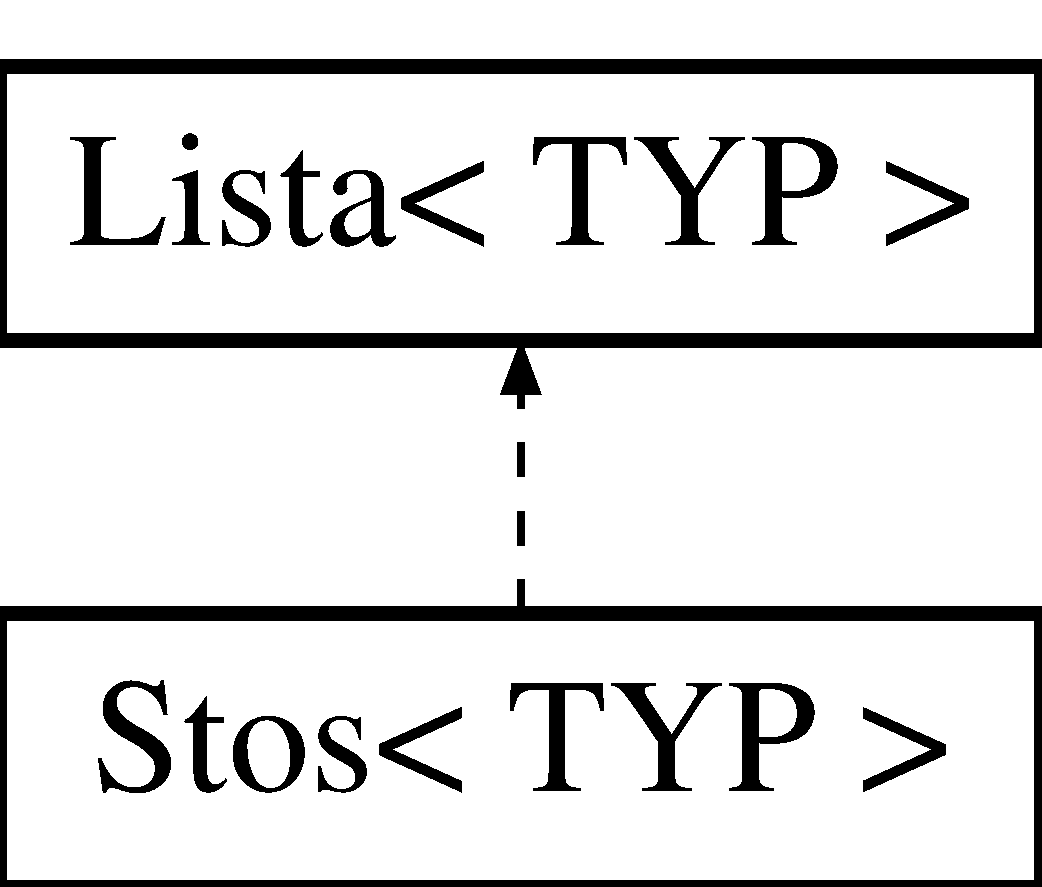
\includegraphics[height=2.000000cm]{class_stos}
\end{center}
\end{figure}
\subsection*{Metody publiczne}
\begin{DoxyCompactItemize}
\item 
\hypertarget{class_stos_a773cf22cb5c67bda0d2878a1ec8bc363}{void {\bfseries P\-U\-S\-H} (T\-Y\-P liczba)}\label{class_stos_a773cf22cb5c67bda0d2878a1ec8bc363}

\item 
\hypertarget{class_stos_ab8b0ecec7cbe0ae761bfee9d9e47d5d4}{int {\bfseries P\-O\-P} ()}\label{class_stos_ab8b0ecec7cbe0ae761bfee9d9e47d5d4}

\item 
\hypertarget{class_stos_a8f1c40b779a699c84b20eeb59ca67f06}{void {\bfseries S\-H\-O\-W} ()}\label{class_stos_a8f1c40b779a699c84b20eeb59ca67f06}

\item 
\hypertarget{class_stos_a6ff0d2aa5946c0dc413e3236ca99fd26}{unsigned int {\bfseries S\-I\-Z\-E} ()}\label{class_stos_a6ff0d2aa5946c0dc413e3236ca99fd26}

\end{DoxyCompactItemize}
\subsection*{Dodatkowe Dziedziczone Składowe}


\subsection{Opis szczegółowy}
\subsubsection*{template$<$typename T\-Y\-P$>$class Stos$<$ T\-Y\-P $>$}

Klasa \hyperlink{class_stos}{Stos}. 

Klasa ta modeluje nam \hyperlink{class_stos}{Stos} Składa się z pól klasy \hyperlink{class_lista}{Lista} ktore zostania uzyte oraz metod P\-U\-S\-H, P\-O\-P, S\-I\-Z\-E, S\-H\-O\-W Klasa w calosci wykorzystuje implementacje listy 

Dokumentacja dla tej klasy została wygenerowana z pliku\-:\begin{DoxyCompactItemize}
\item 
/home/mateusz/git/209365/\-Lab3/prj/inc/\hyperlink{_stos_8hh}{Stos.\-hh}\end{DoxyCompactItemize}

\hypertarget{class_timer}{\section{Dokumentacja klasy Timer}
\label{class_timer}\index{Timer@{Timer}}
}


Klasa do pomiaru różnicy czasów.  




{\ttfamily \#include $<$Timer.\-hh$>$}

\subsection*{Metody publiczne}
\begin{DoxyCompactItemize}
\item 
\hyperlink{class_timer_a5f16e8da27d2a5a5242dead46de05d97}{Timer} ()
\begin{DoxyCompactList}\small\item\em Konstruktor zerujący parametry. \end{DoxyCompactList}\item 
void \hyperlink{class_timer_aa8c887576ec3b0d68c10ebf4097c367c}{start\-Timer} ()
\begin{DoxyCompactList}\small\item\em Zmierzenie czasu rozpoczęcia pomiaru. \end{DoxyCompactList}\item 
void \hyperlink{class_timer_a27f97da1b1d19ad74a847703ca25c455}{stop\-Timer} ()
\begin{DoxyCompactList}\small\item\em Zmierzenie czasu zakończenia pomiaru. \end{DoxyCompactList}\item 
double \hyperlink{class_timer_afa5d5cd3dab1aa6a67278dffd6a42dbf}{diff\-Time\-Ms} ()
\begin{DoxyCompactList}\small\item\em Funkcja zwracająca różnice czasu pomiędzy czasem rozpoczęcia i zakończenia pomiaru. \end{DoxyCompactList}\end{DoxyCompactItemize}


\subsection{Opis szczegółowy}
Klasa do pomiaru różnicy czasów. 

Klasa pozwala na pomiar czasów w danych momentach oraz na zwrócenie czasu, który upłynał pomiędzy tymi momentami 

\subsection{Dokumentacja konstruktora i destruktora}
\hypertarget{class_timer_a5f16e8da27d2a5a5242dead46de05d97}{\index{Timer@{Timer}!Timer@{Timer}}
\index{Timer@{Timer}!Timer@{Timer}}
\subsubsection[{Timer}]{\setlength{\rightskip}{0pt plus 5cm}Timer\-::\-Timer (
\begin{DoxyParamCaption}
{}
\end{DoxyParamCaption}
)}}\label{class_timer_a5f16e8da27d2a5a5242dead46de05d97}


Konstruktor zerujący parametry. 

Konstruktor ten odpowiada za zerowania zmięnnych startu i stopu w celu możliwości późniejszego sprawdzenia, czy pomiary czasu konieczne do wyznaczenia różnicy zostały zrealizowane. 

\subsection{Dokumentacja funkcji składowych}
\hypertarget{class_timer_afa5d5cd3dab1aa6a67278dffd6a42dbf}{\index{Timer@{Timer}!diff\-Time\-Ms@{diff\-Time\-Ms}}
\index{diff\-Time\-Ms@{diff\-Time\-Ms}!Timer@{Timer}}
\subsubsection[{diff\-Time\-Ms}]{\setlength{\rightskip}{0pt plus 5cm}double Timer\-::diff\-Time\-Ms (
\begin{DoxyParamCaption}
{}
\end{DoxyParamCaption}
)}}\label{class_timer_afa5d5cd3dab1aa6a67278dffd6a42dbf}


Funkcja zwracająca różnice czasu pomiędzy czasem rozpoczęcia i zakończenia pomiaru. 

Różnica czasu zwracana jest w milisekundach.

\begin{DoxyPrecond}{Warunek wstępny}
Czas zkończenia pomiaru musi być większy (późniejszy) od czasu jego rozpoczęcia
\end{DoxyPrecond}
\begin{DoxyReturn}{Zwraca}
Zwracana jest różnica czasu zrzutowana do typu double 
\end{DoxyReturn}
\hypertarget{class_timer_aa8c887576ec3b0d68c10ebf4097c367c}{\index{Timer@{Timer}!start\-Timer@{start\-Timer}}
\index{start\-Timer@{start\-Timer}!Timer@{Timer}}
\subsubsection[{start\-Timer}]{\setlength{\rightskip}{0pt plus 5cm}void Timer\-::start\-Timer (
\begin{DoxyParamCaption}
{}
\end{DoxyParamCaption}
)}}\label{class_timer_aa8c887576ec3b0d68c10ebf4097c367c}


Zmierzenie czasu rozpoczęcia pomiaru. 

Funkcja zapamiętuje bierzący czas, jako czas rozpoczęcia pomiaru. \hypertarget{class_timer_a27f97da1b1d19ad74a847703ca25c455}{\index{Timer@{Timer}!stop\-Timer@{stop\-Timer}}
\index{stop\-Timer@{stop\-Timer}!Timer@{Timer}}
\subsubsection[{stop\-Timer}]{\setlength{\rightskip}{0pt plus 5cm}void Timer\-::stop\-Timer (
\begin{DoxyParamCaption}
{}
\end{DoxyParamCaption}
)}}\label{class_timer_a27f97da1b1d19ad74a847703ca25c455}


Zmierzenie czasu zakończenia pomiaru. 

Funkcja zapamiętuje bierzący czas, jako czas zakończenia pomiaru. 

Dokumentacja dla tej klasy została wygenerowana z plików\-:\begin{DoxyCompactItemize}
\item 
/home/mateusz/git/209365/\-Lab3/prj/inc/\hyperlink{_timer_8hh}{Timer.\-hh}\item 
/home/mateusz/git/209365/\-Lab3/prj/src/\hyperlink{_timer_8cpp}{Timer.\-cpp}\end{DoxyCompactItemize}

\chapter{Dokumentacja plików}
\hypertarget{_benchmark_8hh}{\section{Dokumentacja pliku /home/mateusz/git/209365/\-Lab3/prj/inc/\-Benchmark.hh}
\label{_benchmark_8hh}\index{/home/mateusz/git/209365/\-Lab3/prj/inc/\-Benchmark.\-hh@{/home/mateusz/git/209365/\-Lab3/prj/inc/\-Benchmark.\-hh}}
}


Deklaracja i definicja (razem, bo szablon) klasy \hyperlink{class_benchmark}{Benchmark}.  


{\ttfamily \#include \char`\"{}../inc/\-Lista.\-hh\char`\"{}}\\*
{\ttfamily \#include \char`\"{}../inc/quick\-\_\-sort.\-hh\char`\"{}}\\*
{\ttfamily \#include \char`\"{}../inc/merge\-\_\-sort.\-hh\char`\"{}}\\*
{\ttfamily \#include \char`\"{}../inc/\-Timer.\-hh\char`\"{}}\\*
{\ttfamily \#include $<$iostream$>$}\\*
{\ttfamily \#include $<$cstdlib$>$}\\*
{\ttfamily \#include $<$cstdio$>$}\\*
{\ttfamily \#include $<$ctime$>$}\\*
{\ttfamily \#include $<$string$>$}\\*
\subsection*{Komponenty}
\begin{DoxyCompactItemize}
\item 
class \hyperlink{class_benchmark}{Benchmark$<$ T $>$}
\begin{DoxyCompactList}\small\item\em Klasa do przeprowadzenia testów na kontenerach danych. \end{DoxyCompactList}\end{DoxyCompactItemize}


\subsection{Opis szczegółowy}
Deklaracja i definicja (razem, bo szablon) klasy \hyperlink{class_benchmark}{Benchmark}. \hyperlink{_benchmark_8hh}{Benchmark.\-hh} 
\hypertarget{_kolejka_8hh}{\section{Dokumentacja pliku /home/mateusz/git/209365/\-Lab3/prj/inc/\-Kolejka.hh}
\label{_kolejka_8hh}\index{/home/mateusz/git/209365/\-Lab3/prj/inc/\-Kolejka.\-hh@{/home/mateusz/git/209365/\-Lab3/prj/inc/\-Kolejka.\-hh}}
}


Definicja klasy \hyperlink{class_kolejka}{Kolejka}.  


{\ttfamily \#include $<$iostream$>$}\\*
{\ttfamily \#include \char`\"{}Lista.\-hh\char`\"{}}\\*
\subsection*{Komponenty}
\begin{DoxyCompactItemize}
\item 
class \hyperlink{class_kolejka}{Kolejka$<$ T\-Y\-P $>$}
\begin{DoxyCompactList}\small\item\em Klasa \hyperlink{class_kolejka}{Kolejka}. \end{DoxyCompactList}\end{DoxyCompactItemize}


\subsection{Opis szczegółowy}
Definicja klasy \hyperlink{class_kolejka}{Kolejka}. Plik zawiera definicje klasy \hyperlink{class_kolejka}{Kolejka}, ktora bedzie struktura naszych danych. Klasa ta posiada szablon, dzieki czemu mozemy pracowac na roznych typach danych 
\hypertarget{_lista_8hh}{\section{Dokumentacja pliku /home/mateusz/git/209365/\-Lab3/prj/inc/\-Lista.hh}
\label{_lista_8hh}\index{/home/mateusz/git/209365/\-Lab3/prj/inc/\-Lista.\-hh@{/home/mateusz/git/209365/\-Lab3/prj/inc/\-Lista.\-hh}}
}


Definicja klasy \hyperlink{class_lista}{Lista}.  


{\ttfamily \#include $<$iostream$>$}\\*
\subsection*{Komponenty}
\begin{DoxyCompactItemize}
\item 
class \hyperlink{class_lista}{Lista$<$ T\-Y\-P $>$}
\begin{DoxyCompactList}\small\item\em Klasa \hyperlink{class_lista}{Lista}. \end{DoxyCompactList}\end{DoxyCompactItemize}


\subsection{Opis szczegółowy}
Definicja klasy \hyperlink{class_lista}{Lista}. Plik zawiera definicje klasy \hyperlink{class_lista}{Lista} ktora bedzie struktura danych oparta na tablicy dynamicznej 
\hypertarget{_stos_8hh}{\section{Dokumentacja pliku /home/mateusz/git/209365/\-Lab3/prj/inc/\-Stos.hh}
\label{_stos_8hh}\index{/home/mateusz/git/209365/\-Lab3/prj/inc/\-Stos.\-hh@{/home/mateusz/git/209365/\-Lab3/prj/inc/\-Stos.\-hh}}
}


Definicja klasy \hyperlink{class_stos}{Stos}.  


{\ttfamily \#include $<$iostream$>$}\\*
{\ttfamily \#include \char`\"{}Lista.\-hh\char`\"{}}\\*
\subsection*{Komponenty}
\begin{DoxyCompactItemize}
\item 
class \hyperlink{class_stos}{Stos$<$ T\-Y\-P $>$}
\begin{DoxyCompactList}\small\item\em Klasa \hyperlink{class_stos}{Stos}. \end{DoxyCompactList}\end{DoxyCompactItemize}


\subsection{Opis szczegółowy}
Definicja klasy \hyperlink{class_stos}{Stos}. Plik zawiera definicje klasy \hyperlink{class_stos}{Stos}, ktora bedzie struktura naszych danych. Klasa ta posiada szablon, dzieki czemu mozemy pracowac na roznych typach danych 
\hypertarget{_timer_8hh}{\section{Dokumentacja pliku /home/mateusz/git/209365/\-Lab3/prj/inc/\-Timer.hh}
\label{_timer_8hh}\index{/home/mateusz/git/209365/\-Lab3/prj/inc/\-Timer.\-hh@{/home/mateusz/git/209365/\-Lab3/prj/inc/\-Timer.\-hh}}
}


Plik zawierający deklaracje klasy \hyperlink{class_timer}{Timer} służącej do pomiaru różnicy czasów.  


{\ttfamily \#include $<$ctime$>$}\\*
\subsection*{Komponenty}
\begin{DoxyCompactItemize}
\item 
class \hyperlink{class_timer}{Timer}
\begin{DoxyCompactList}\small\item\em Klasa do pomiaru różnicy czasów. \end{DoxyCompactList}\end{DoxyCompactItemize}


\subsection{Opis szczegółowy}
Plik zawierający deklaracje klasy \hyperlink{class_timer}{Timer} służącej do pomiaru różnicy czasów. Timer.\-h 
\hypertarget{_timer_8cpp}{\section{Dokumentacja pliku /home/mateusz/git/209365/\-Lab3/prj/src/\-Timer.cpp}
\label{_timer_8cpp}\index{/home/mateusz/git/209365/\-Lab3/prj/src/\-Timer.\-cpp@{/home/mateusz/git/209365/\-Lab3/prj/src/\-Timer.\-cpp}}
}


Plik zawierający definicje funkcji klasy \hyperlink{class_timer}{Timer} służącej do pomiaru różnicy czasów.  


{\ttfamily \#include \char`\"{}../inc/\-Timer.\-hh\char`\"{}}\\*
{\ttfamily \#include $<$iostream$>$}\\*


\subsection{Opis szczegółowy}
Plik zawierający definicje funkcji klasy \hyperlink{class_timer}{Timer} służącej do pomiaru różnicy czasów. \hyperlink{_timer_8cpp}{Timer.\-cpp} 
%--- End generated contents ---

% Index
\newpage
\phantomsection
\addcontentsline{toc}{chapter}{Indeks}
\printindex

\end{document}
